\documentclass{beamer}
\usetheme[block = fill, titleformat title = allcaps, titleformat subtitle  = smallcaps,
progressbar = foot, background = light]{metropolis}           % Use metropolis theme
\usepackage{pgfplots}
\usepackage{appendixnumberbeamer}
\usepackage{booktabs}
\usepackage{amsmath, array}
\usetikzlibrary{arrows.meta,positioning, shapes, backgrounds}

\usepackage[sortcites=false,style=authoryear-comp,bibencoding=utf8, natbib=true, firstinits=true, maxcitenames=2, maxbibnames = 99, uniquename=false, backend=bibtex, useprefix=true, backref=false,doi=false,isbn=false,url=false,dashed=true]{biblatex}
\setlength\bibhang{20pt}
\bibliography{../../paper/references.bib}
\AtEveryBibitem{%
	\clearfield{day}%
	\clearfield{month}%
	\clearfield{endday}%
	\clearfield{endmonth}%
}
\AtBeginBibliography{\footnotesize}

\makeatletter
\let\save@measuring@true\measuring@true
\def\measuring@true{%
	\save@measuring@true
	\def\beamer@sortzero##1{\beamer@ifnextcharospec{\beamer@sortzeroread{##1}}{}}%
	\def\beamer@sortzeroread##1<##2>{}%
	\def\beamer@finalnospec{}%
}
\makeatother

\title{Housing market and migration revisited}
\subtitle{A multilevel gravity model for Dutch regions}
\date{August 25, 2020}
\author{Thomas de Graaff}
\institute{Vrije Universiteit Amsterdam\\Tinbergen Institute Amsterdam}
\begin{document}
\maketitle


\begin{frame}{Housing market and interregional migration: why bother?}
   	\begin{itemize}
   		\item Dutch housing market: tight and regulated
   		\begin{itemize}
   			\item large \alert{shortage} of housing
   			\item large yearly prices \alert{increases} ($\approx 5\%-9\%$ annually)
   			\item decrease in housing \alert{transactions}
   			\item large \alert{regional} variation\newline \pause
   		\end{itemize}
            \item Regional Dutch population projections (PEARL)  $\longrightarrow$ difficulties with \alert{interregional} migration
            \begin{itemize}
            \item especially long-distance migration  
            \item changes in local housing supply as input \newline \pause
            \end{itemize}
   		\item Large literature of \alert{external} effects of home-ownership \footnotesize{\citep{dietz2003social}}
   		\begin{itemize}
   			\item \alert{negative}: migration (by increased moving costs) and on aggregate labour market performance \footnotesize{\citep{oswald1996conjecture,oswald1999housing}}
   		\end{itemize}
   	\end{itemize}
\end{frame}

\begin{frame}{My contributions to the literature}
  \begin{itemize}
  \item Large empirical (economic) literature on impact home-ownership as drivers of interregional migration, but:
    \begin{itemize}
    \item usually concerns \alert{marginal} effect of home-ownership
    \item less attention to \alert{predictions} for the whole network\newline
    \end{itemize}
  \item Literature on impact of social renting on migration flows is
    scarce \footnotesize{\citep{de2009homeownership} }
	\begin{itemize}
        \item In the Netherlands social renting is a large phenomenon
          ($\approx$ 24\% of total housing stock)
        \item Social renting rights only valid \alert{within} city
        \item Social renting is an \alert{urban} phenomenon (e.g. $\approx$
          40--50\% in Amsterdam) 
        \end{itemize}
\end{itemize}
\end{frame}

\begin{frame}{So, this paper}
  \begin{description}
  \item[Does what?] \alert{Revisits} the impact of housing market
    structure (with focus on social renting) on Dutch interregional
    migration flows using a \alert{multilevel} gravity model
    \begin{footnotesize}
	\begin{itemize}
	  \item \footnotesize UK context by \citet{congdon2010random}
	  \item \footnotesize social relations model \emph{cf.}
		\citet{koster2014food}
		\item \footnotesize \emph{Statistical Rethinking} from \citet{mcelreath2020statistical}
		\item \footnotesize \texttt{ggplot2} code from \href{https://bookdown.org/content/4857/}{Solomon Kurz} (2020) \newline
	\end{itemize}
  \end{footnotesize}
	\item[Aim] To \alert{model} the impact of housing market structure on the whole \alert{network} of interregional migration flows
  \end{description}
\end{frame}


\begin{frame}[fragile]{Why a \textbf{multilevel} approach for migration?}
There are at least two \alert{levels} in migration (I use three) \pause
\begin{description}
	\item[Observed migration \alert{flows}] Migration between $i$ and $j$ with friction (e.g., distance) attributes (obs = $R^2 - R$)
		\begin{figure}	
		\begin{tikzpicture}[scale=0.90, thick]
		
		\tikzstyle{orig}=[rectangle, rounded corners, thin, fill=green!20, text=black, draw, minimum width=2cm]
		\tikzstyle{dest}=[rectangle, rounded corners, thin, fill=red!20, text=black, draw, minimum width=2cm]
	\tikzstyle{var}=[rectangle, rounded corners, thin, fill=black!10, text=black, draw, minimum width = 0.6cm, minimum height = 0.4cm]
		\node[orig] (o1) at (0,0)  {\textsc{region$_i$}};
		\node[dest] (d1) at (6,0)  {\textsc{region$_j$}};	
		% Migration links
		\draw[-latex, black, thick] (1.5,0) -- (4.5, 0);
		\node[var] (m) at (3,0)  {\scriptsize \textsc{$\mathbf{X}_{ij}$}};

		\end{tikzpicture}
	\end{figure}\pause
	\item[Observed push \& pull factors] Attributes of $i$ and $j$ (obs $= R$)
		\begin{figure}	
	\begin{tikzpicture}[scale=0.90, thick]
	
	\tikzstyle{orig}=[rectangle, rounded corners, thin, fill=green!20, text=black, draw, minimum width=2cm]
	\tikzstyle{dest}=[rectangle, rounded corners, thin, fill=red!20, text=black, draw, minimum width=2cm]
	\tikzstyle{var}=[rectangle, rounded corners, thin, fill=black!10, text=black, draw, minimum width = 0.6cm, minimum height = 0.4cm]
	\node[orig] (o1) at (0,0)  {\textsc{region$_i$}};
	\node[dest] (d1) at (6,0)  {\textsc{region$_j$}};	

	\node[var] (v1) at (0,-1.2)  {\scriptsize \textsc{$\mathbf{X}_i$}};
	\node[var] (v3) at (6,-1.2)  {\scriptsize \textsc{$\mathbf{X}_j$} };

	\draw[-latex, thick, black] (v1) -- (o1);
	\draw[-latex, thick, black] (v3) -- (d1);
	
	\end{tikzpicture}
\end{figure}\pause	
	\item[Observed flows between region \alert{dyads}] migration from $i \rightarrow j$ is correlated with migration from $j \rightarrow i$ (obs $= \frac{R^{2}- R}{2}$)
			\begin{figure}	
		\begin{tikzpicture}[scale=0.90, thick]
		
		\tikzstyle{orig}=[rectangle, rounded corners, thin, fill=green!20, text=black, draw, minimum width=2cm]
		\tikzstyle{dest}=[rectangle, rounded corners, thin, fill=red!20, text=black, draw, minimum width=2cm]
		\node[orig] (o1) at (0,0)  {\textsc{region$_i$}};
		\node[dest] (d1) at (6,0)  {\textsc{region$_j$}};	
		% Migration links
		\draw[-latex, black, thick] (1.5,0.15) -- (4.5, 0.15);
		\draw[-latex, black, thick] (4.5,-0.15) -- (1.5, -0.15);		
		
		\end{tikzpicture}
	\end{figure}
\end{description}
\end{frame}

\begin{frame}{Why a Bayesian multilevel approach?}
\begin{itemize}
	\item Hierarchical, mixed effects, varying intercept/parameter, shrinkage, partial pooling models\pause
	\item Increasingly used for model \alert{performance} and \alert{flexibility} \pause
    \item \alert{Simultaneous} modeling at various levels (e.g., cities, regions, flows, individuals) 
    \begin{itemize}
    	\item no two-stage models anymore 
    	\item precision (standard errors) is correct\pause
    \end{itemize}
	\item \alert{Partial pooling}: For example, origin specific effects are drawn from a distribution: usually $\sim \text{ Normal}(\alpha, \sigma)$
	\begin{itemize}
		\item $\sigma \longrightarrow 0$ : complete pooling
		\item $\sigma \longrightarrow \infty$ : no pooling (fixed effects)
	\end{itemize}
\end{itemize}
\end{frame}

\begin{frame}{Data: migrations flows in 2018}
	\begin{center}
		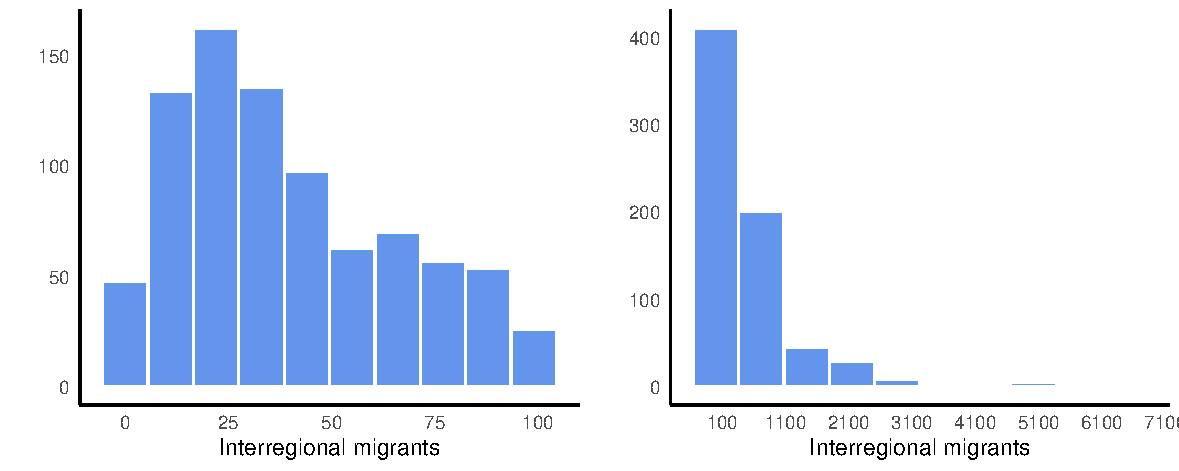
\includegraphics[width=0.8\textwidth]{../../fig/hist_mig_corop}      
	\end{center}
\begin{itemize}
	\item Panel for the period 2012--2018
	\item Migration flows \alert{between} 40 Dutch regions ($1,560$ flows per year)
	\item Variance $\gg$ mean: \alert{over-dispersion}
\end{itemize}
\end{frame}

\begin{frame}{Data: regional housing structure in 2018}
\begin{center}
	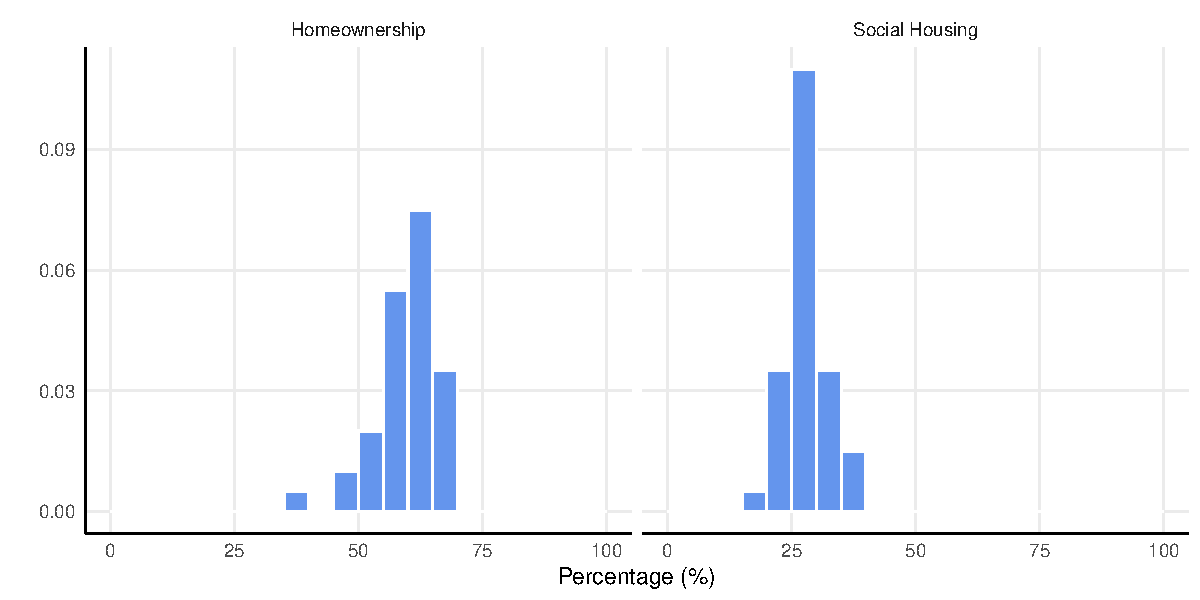
\includegraphics[width=0.8\textwidth]{../../fig/hist_housing_corop}
\end{center}
\begin{itemize}
	\item Positive correlation between population and share social renting ($0.46$)
	\item Negative correlation between share social renting and share home-ownership ($-0.88)$
\end{itemize}
\end{frame}

\begin{frame}{Data: regional housing structure in 2018 (cont.)}
		\begin{columns}
	\begin{column}{0.5\textwidth}
	  \begin{center}
		\begin{figure}
		  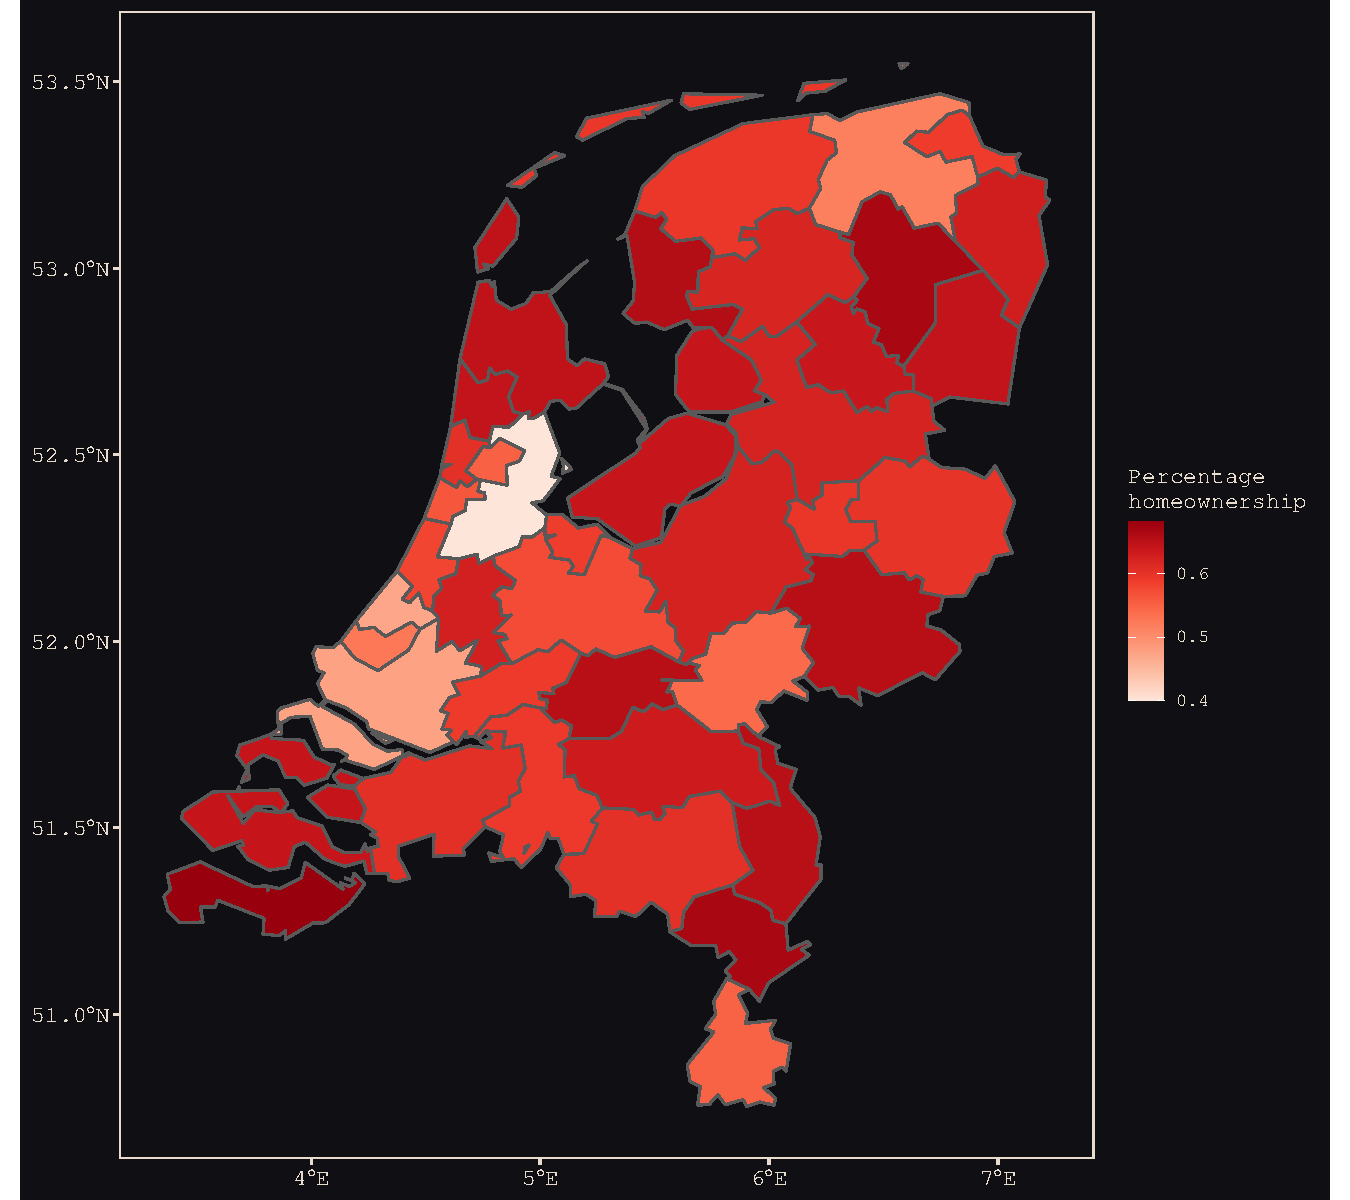
\includegraphics[width=1.1\textwidth]{../../fig/p_homeown}
		  \caption{Share of homeownership}
		  \end{figure}
		\end{center}
	\end{column}
	\begin{column}{0.5\textwidth}
		\begin{center}
		  \begin{figure}
		  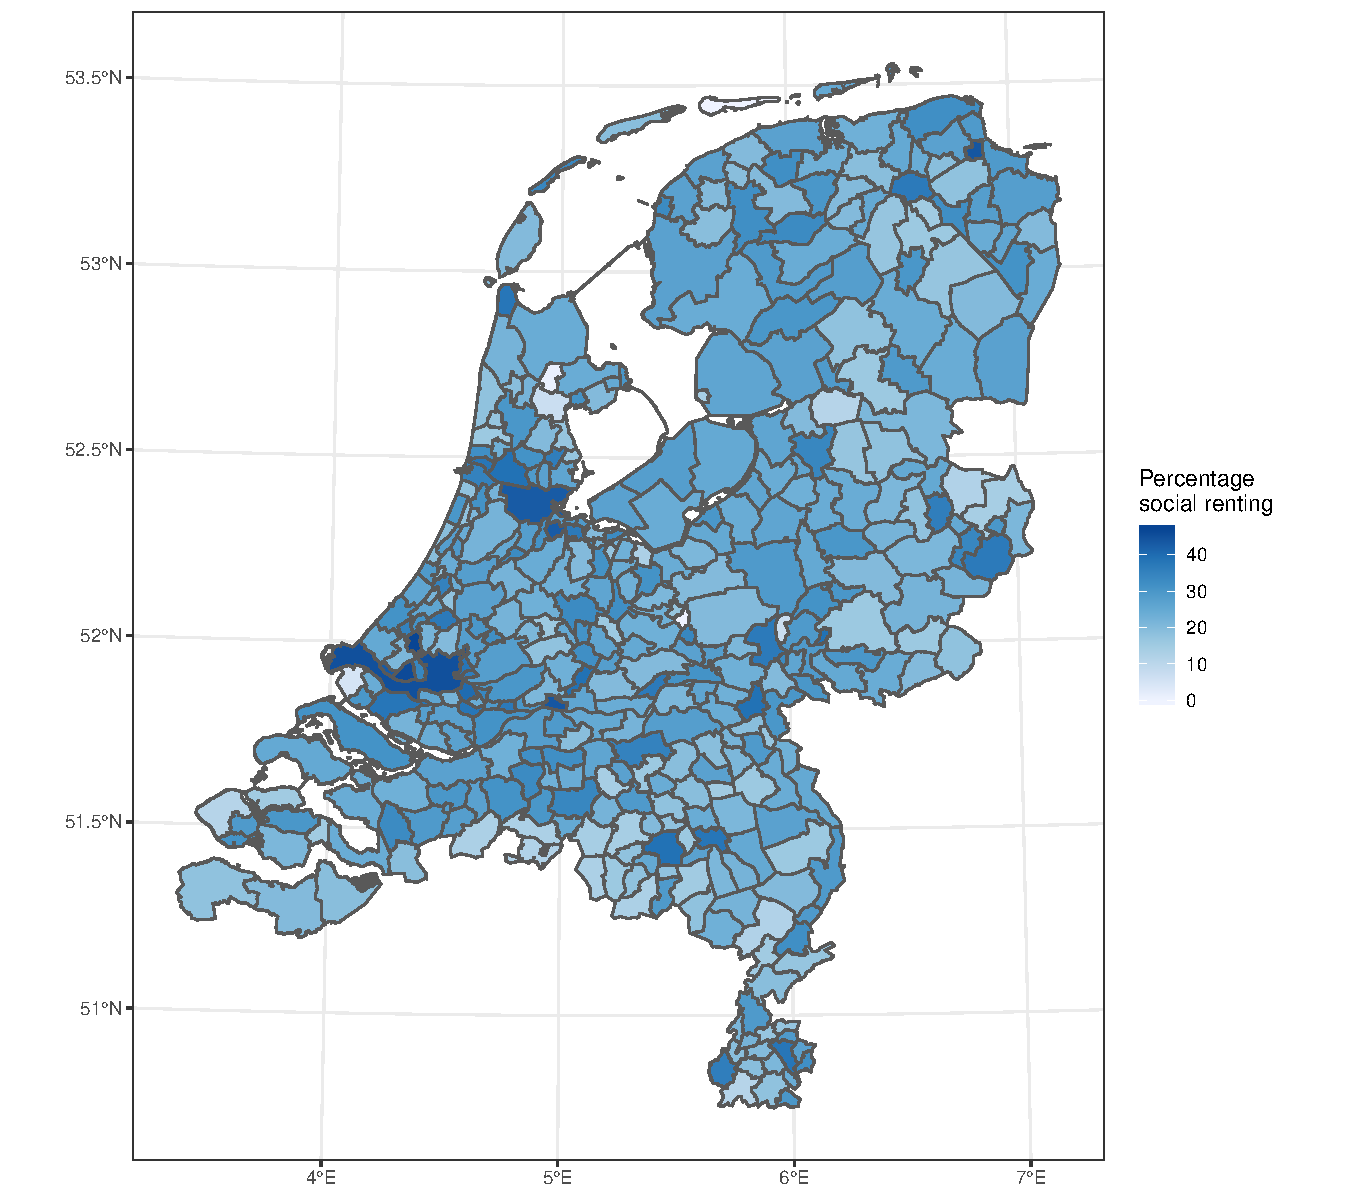
\includegraphics[width=1.1\textwidth]{../../fig/p_socrent}
		  \caption{Share of social renting}
		  \end{figure}
		\end{center}
	\end{column}
\end{columns}
\end{frame}


\begin{frame}{Modeling framework: traditional gravity modeling}
	\begin{equation*}
	\log(\text{Migrants}_{ij}) = o_i + d_j + \gamma\log(\text{dist}_{ij}) + \epsilon_{ij}
	\label{eq:gravfixed}
	\end{equation*} 
	
	Origin and destination specific \alert{fixed} effects for multilateral resistance  \citep{anderson2003gravity}, but:
	\begin{itemize}
		\item what about \alert{zeros} in $\text{Migrants}_{ij}$?
		\item how to incorporate \alert{housing} structure in the presence of $o_i$ and $d_j$?
		\item \alert{over-dispersion} and \alert{heteroskedasticity} \footnotesize{\citep{silva2006log} }
	\end{itemize}
\end{frame}

\begin{frame}{Poisson versus negative binomial\footnote{
			\emph{We urge researchers to resist the siren song of the Negative
			Binomial \footnotesize{ \citep{head2014gravity}} }
			}}
	
	\begin{itemize}
		\item Counts of migrants\newline 
		\item 	With Poisson \& regional effects of origin and destination the following origin and destination \alert{constraints} automatically hold
		$$
		\sum_{j=1}^{R} {\widehat{\text{Migrants} }_{ij} } = O_i \qquad \sum_{i=1}^{R} {\widehat{\text{Migrants} }_{ij} } = D_j
		$$

	\item  Does not apply with negative binomial \newline
	\item Multilevel model accounts for dispersion
		\end{itemize}

\end{frame}

\begin{frame}[fragile]{Modeling framework: multilevel gravity modeling}
\begin{small}
  \begin{align}
	\text{Migrants}_{ij} \sim & \text{ Poisson}(\lambda_{ij}) \notag \\
	\text{Migrants}_{ji} \sim & \text{ Poisson}(\lambda_{ji}) \tag{\footnotesize \color{blue} flow of migrants} \\ \pause
	\log(\lambda_{ij}) =  & \: \alpha + o_{i} + d_{j} + \text{dyad}_{ij} +\tag{\footnotesize
							\color{blue} correlation structure}  \\ \pause
							  & \: \mathbf{X}_{i}  \beta_{i}+ \mathbf{X}_{j} \beta_{j}  \tag{\footnotesize \color{blue} explanatory variables}  \\ \pause
	\log(\lambda_{ji}) =  & \: \alpha + o_{j} + d_{i} + \text{dyad}_{ji} + \notag \\
							  & \: \mathbf{X}_{j}  \beta_{i}+ \mathbf{X}_{i} \beta_{j} \notag  \\ \pause
	\left(\begin{matrix} 
		o_{i} \\
		d_{i}
	\end{matrix}\right) \sim& \text{ MVNormal}\left( \left( \begin{matrix}
	0 \\
	0 
	\end{matrix}\right) , \left(\begin{matrix}
	\sigma_o^2 & \sigma_o \sigma_d \rho \\
	 \sigma_o \sigma_d \rho  & \sigma_d^2
	\end{matrix}\right) \right)  \tag{\footnotesize \color{blue} varying region effects}  \\ \pause 	\left(\begin{matrix} 
		\text{dyad}_{ij} \\
		\text{dyad}_{ji}
	\end{matrix}\right) \sim& \text{ MVNormal}\left( \left( \begin{matrix}
	0 \\
	0 
	\end{matrix}\right) , \left(\begin{matrix}
	\sigma_{\text{dyad}}^2 & \sigma_{\text{dyad}}^2 \rho_{\text{dyad}} \\
	 \sigma_{\text{dyad}}^2 \rho_{\text{dyad}}  & \sigma_{\text{dyad}}^2
	\end{matrix}\right) \right)  \tag{\footnotesize \color{blue} varying dyad effects}
	\end{align}
\end{small}
\end{frame}





\begin{frame}{Estimation results}
		\begin{columns}
		\begin{column}{0.5\textwidth}
			\begin{center}
				\begin{small}
			  \begin{tabular}{lrr}
				\toprule
				Parameter & mean & sd \\ 
				\midrule
				Intercept ($\alpha$)      & $4.49$ & 0.15 \\
				log(pop$_i$)   & 0.40 & 0.04  \\
				log(pop$_j$)   & 0.64 & 0.03  \\
				log(home$_i$)  & $1.80$ & 0.10 \\
				log(home$_j$)  & $-0.50$ & 0.09 \\
				log(soc$_i$)   & $0.77$ & 0.07 \\
				log(soc$_j$)   & $0.06$ & 0.07 \\
				log(dist$_{ij})$ & $-1.62$ & 0.03  \\
				\bottomrule
			\end{tabular}
		\end{small}
		\end{center}
		\end{column}
		\begin{column}{0.5\textwidth} 

			\begin{center}
				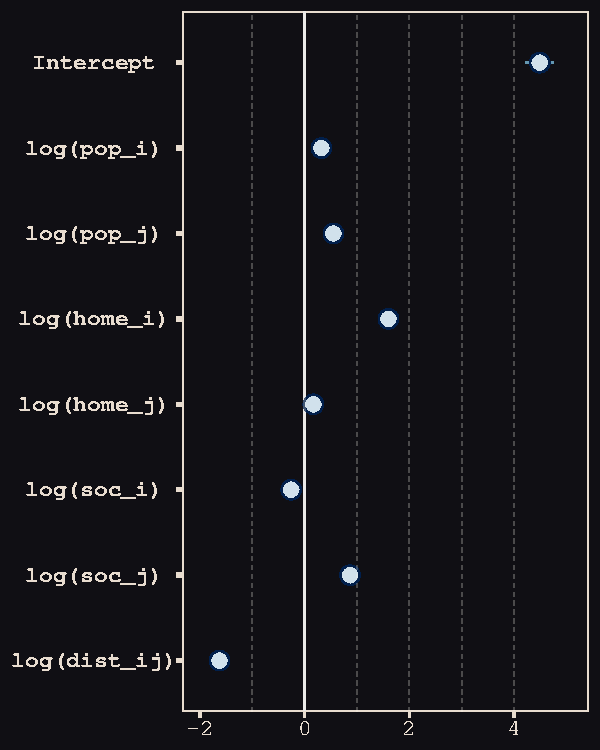
\includegraphics[width=\textwidth]{../../fig/forestplot}      
			\end{center}
		\end{column}
	\end{columns}
\end{frame}



\begin{frame}{Observed versus predicted flows (correlation $\approx 0.99$ )}
\begin{center}
	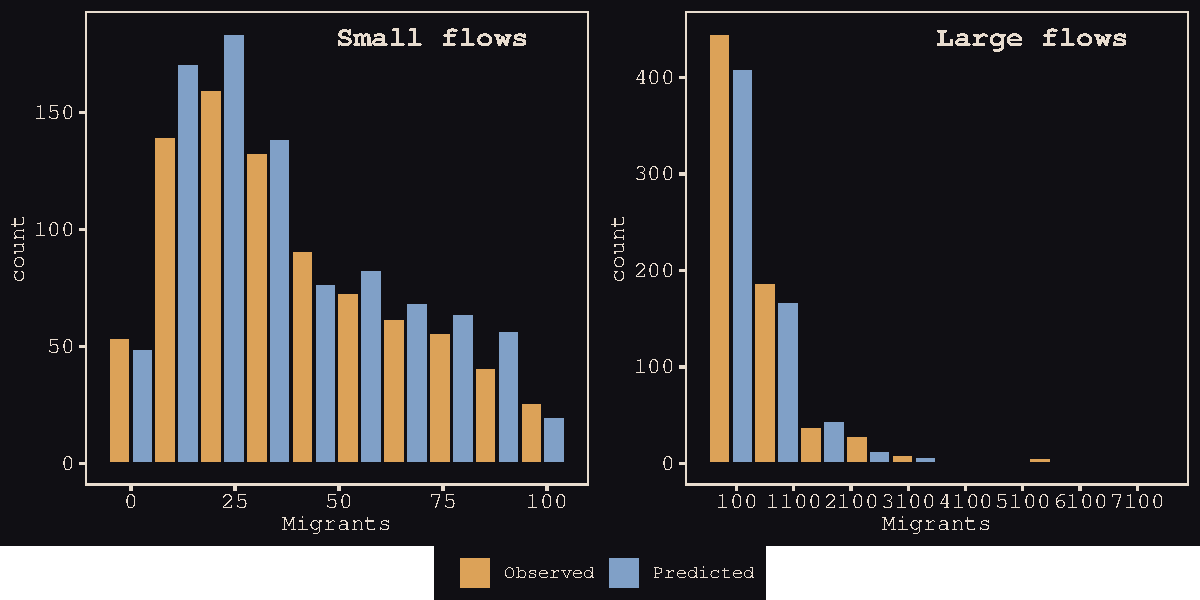
\includegraphics[width=0.9\textwidth]{../../fig/hist_fit}      
\end{center}
\begin{itemize}
	\item \alert{maximum} observed flow: 6,555
	\item \alert{maximum} predicted flow: 4,704
\end{itemize}
\end{frame}

\begin{frame}{Correlation between origin and destination $\rho = 0.88$}
				\begin{center}
		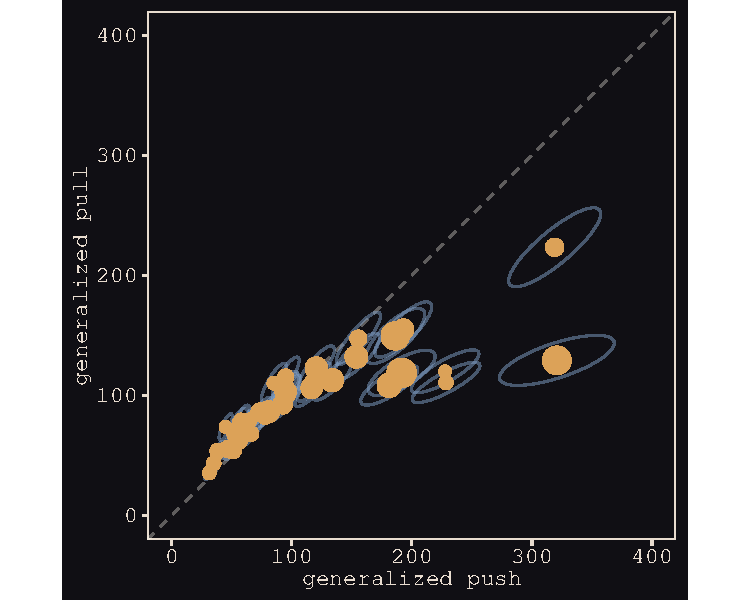
\includegraphics[width=0.9\textwidth]{../../fig/scatter}
	\end{center}
\end{frame}


\begin{frame}{Asymmetric push and pull factors}
		\begin{columns}
	\begin{column}{0.5\textwidth}
		\begin{center}
			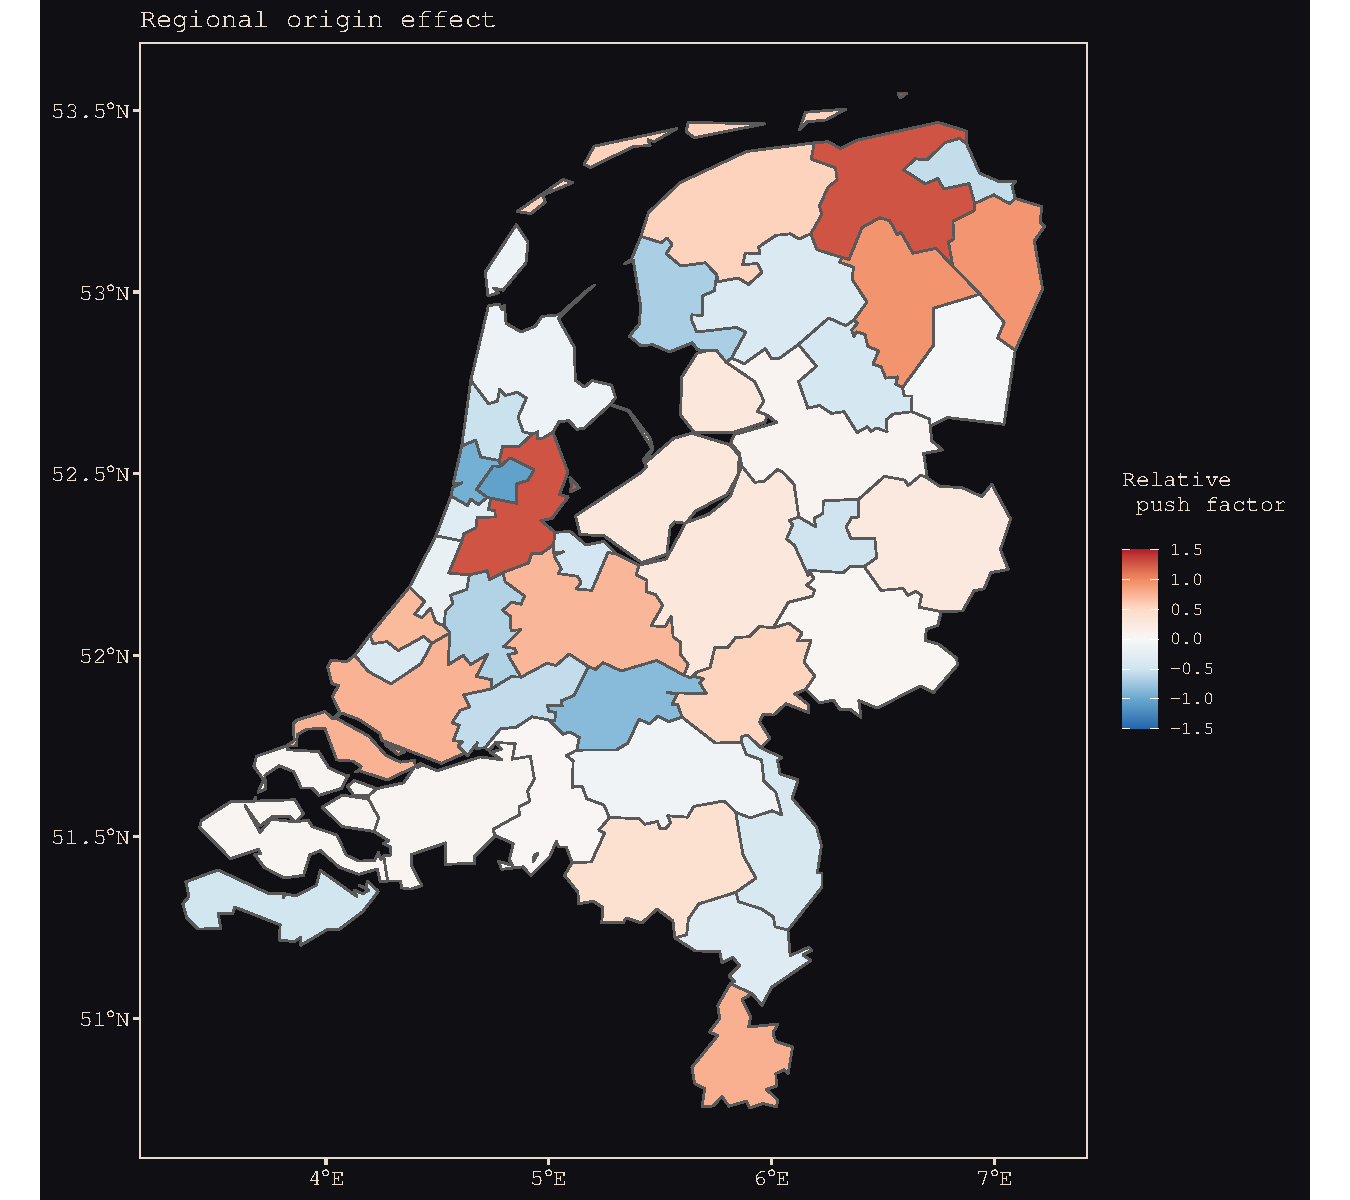
\includegraphics[width=1.1\textwidth]{../../fig/p_coef_out}      
		\end{center}
	\end{column}
	\begin{column}{0.5\textwidth} 	
		\begin{center}
			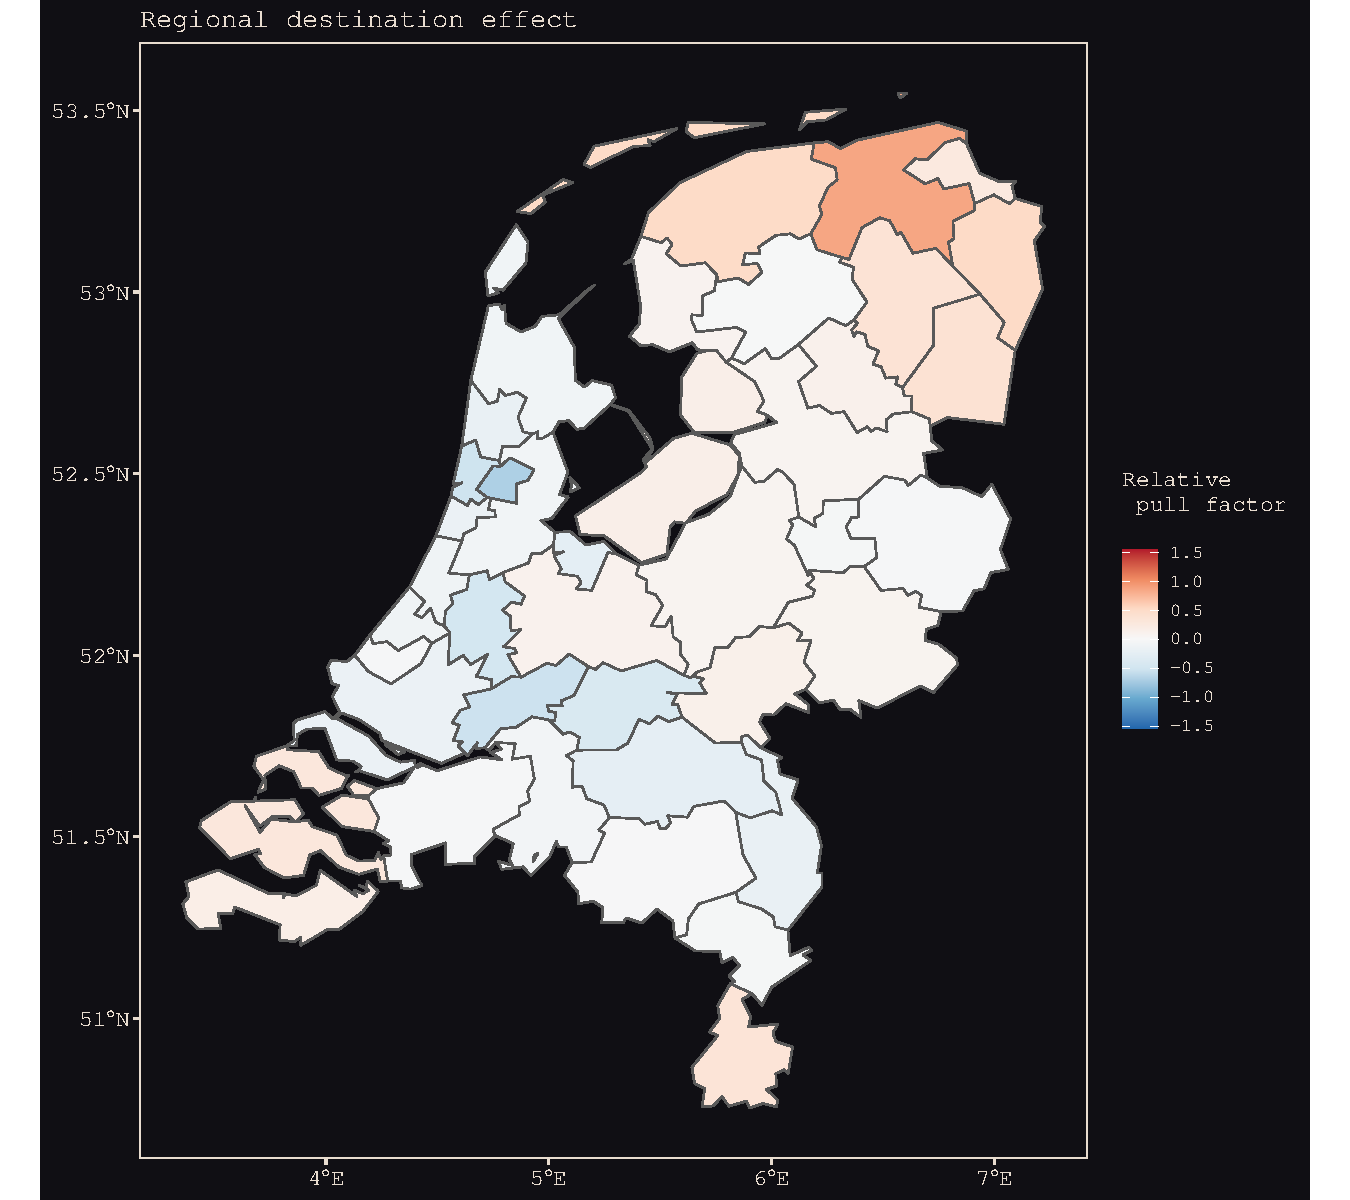
\includegraphics[width=1.1\textwidth]{../../fig/p_coef_in}      
		\end{center}
	\end{column}
\end{columns}
\end{frame}

\begin{frame}{Dyad specific effects $\rho = 0.8$}
				\begin{center}
		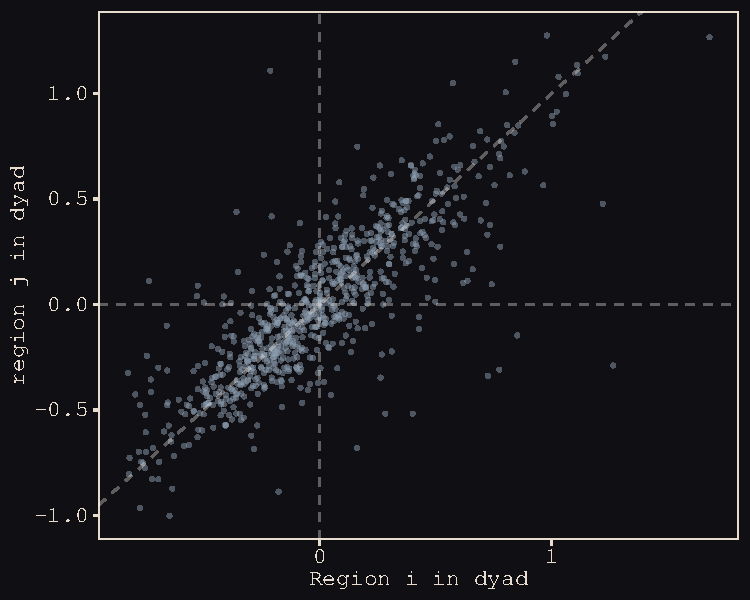
\includegraphics[width=0.9\textwidth]{../../fig/dyad}
	\end{center}
\end{frame}

\begin{frame}{Sensitivity checks}
			\begin{columns}
		\begin{column}{0.5\textwidth}
				Results are \alert{robust} to
				\begin{itemize}
					\item year\pause
					\item interaction effects with population \pause
				  \item inclusion of household size \pause
				  \item spatial autocorrelation in regional effects:
					\begin{eqnarray*}
					  o_{i}, d_{j}& \sim &\text{MVNormal}(0, \mathbf{K})\\
					  \mathbf{K}_{ij} & = & \eta^{2}\exp(-\rho^{2}\mathbf{D}_{ij})
					\end{eqnarray*}
					\pause
				  \end{itemize}
		\end{column}
		\begin{column}{0.5\textwidth}
			\alert{Modest} spatial autocorrelation
			\begin{center}
				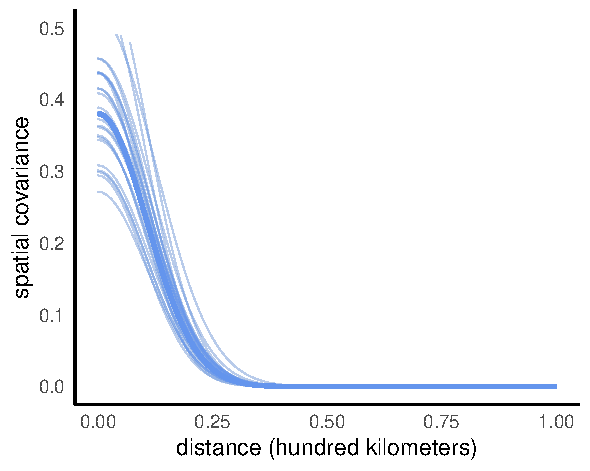
\includegraphics[width=\textwidth]{../../fig/spatial_autocorrelation}
			\end{center}
		\end{column}
	\end{columns}
\end{frame}

\begin{frame}{Conclusions}
\textbf{Flexibel and powerful Bayesian multilevel gravity model}:
\begin{itemize}
  \item housing structure asymmetric impact on migration
  \begin{itemize}
	\item positive on push/negative on pull
	\item push factor large in large cities
  \end{itemize}
	\item impact social renting smaller than homeowership
\citep{boyle1998migration}
	\begin{itemize}
	  \item social housing is like a \alert{different ball game}
	\end{itemize}
	\item tight housing market
\end{itemize}

\textbf{Now what?}
\begin{itemize}
	\item model \alert{performance} is quite good
	\begin{itemize}
	  \item out-of-sample prediction
	  \item \alert{long-distance} migration (dyad effects)
	\end{itemize}
\end{itemize}
\end{frame}

\begin{frame}{Supplementary materials}

Paper, presentation, data and code can be retrieved from the project's GitHub page: 

\begin{center}\url{https://github.com/Thdegraaff/migration\_gravity}\end{center}

\end{frame}

\begin{frame}[standout]
Thank you!
\end{frame}

\appendix

\begin{frame}[allowframebreaks]{References}

		\printbibliography[heading=none]

\end{frame}


\end{document}
